\documentclass[11pt]{article}
\usepackage[margin=1in]{geometry}
\usepackage{amsmath,amssymb}
\usepackage{tikz}
\usetikzlibrary{arrows.meta}

\title{Nonlinear Control Notes: $\dot{x} + x^2 = u$}
\author{}
\date{}

\begin{document}
\maketitle

\section*{The system}
With $u = 0$, the system is
\begin{equation}
  \dot{x} = -x^2 .
  \label{eq:sys}
\end{equation}
The only equilibrium is $x = 0$, since that is the only point where $\dot{x} = 0$.

\section*{Sign of $\dot{x}$}
Because $x^2 \ge 0$, \eqref{eq:sys} gives
\begin{equation}
  \dot{x} = -x^2 \le 0 \quad \text{for all } x .
  \label{eq:sign}
\end{equation}
So $x$ can only decrease or stay where it is, wherever it starts:
\begin{itemize}
  \item $x_0 > 0$: $x$ decreases toward $0$. The state settles back to the equilibrium.
  \item $x_0 < 0$: $x$ also decreases, which takes it \emph{away} from $0$ toward $-\infty$. The further it goes, the larger $x^2$ becomes, so it speeds up as it runs away.
\end{itemize}

\begin{center}
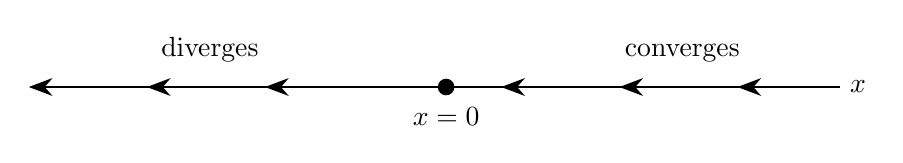
\begin{tikzpicture}[>={Stealth[length=3mm]}]
  \draw[thick] (-5,0) -- (5,0) node[right] {$x$};
  \foreach \s in {-4.5,-3,-1.5} \draw[->,thick] (\s,0) -- (\s-0.8,0);
  \foreach \s in {4.5,3,1.5} \draw[->,thick] (\s,0) -- (\s-0.8,0);
  \fill (0,0) circle (3pt) node[below=4pt] {$x=0$};
  \node[above] at (-3,0.2) {diverges};
  \node[above] at (3,0.2) {converges};
\end{tikzpicture}
\end{center}

Trajectories approach the equilibrium from the right and leave it on the left. This is a \textbf{semi-stable} equilibrium. It is \emph{not} stable, because the smallest negative disturbance sends the state away for good.

\section*{Finite escape time}

\subsection*{Solving the equation}
If $x_0 = 0$, the solution is simply $x(t) = 0$. Otherwise $x(t) \ne 0$ (a trajectory cannot reach the equilibrium in finite time, by uniqueness of solutions), so we may divide \eqref{eq:sys} by $x^2$ and separate variables:
\begin{equation}
  \frac{dx}{dt} = -x^2
  \quad\Longrightarrow\quad
  \frac{dx}{x^2} = -\,dt .
  \label{eq:sep}
\end{equation}
Integrate both sides, the left from $x_0$ to $x(t)$ and the right from $0$ to $t$:
\begin{equation}
  \int_{x_0}^{x(t)} \xi^{-2}\, d\xi = -\int_0^t d\tau .
  \label{eq:int}
\end{equation}
Since $\int \xi^{-2}\,d\xi = -\xi^{-1}$, this evaluates to
\begin{equation}
  \left[-\frac{1}{\xi}\right]_{x_0}^{x(t)} = -\frac{1}{x(t)} + \frac{1}{x_0} = -t .
  \label{eq:eval}
\end{equation}
Solving for $1/x(t)$,
\begin{equation}
  \frac{1}{x(t)} = \frac{1}{x_0} + t = \frac{1 + x_0 t}{x_0},
  \label{eq:recip}
\end{equation}
and inverting gives the solution
\begin{equation}
  \boxed{\,x(t) = \frac{x_0}{1 + x_0 t}\,}
  \label{eq:sol}
\end{equation}

\paragraph{Check.} At $t = 0$, \eqref{eq:sol} gives $x(0) = x_0$. Differentiating,
\begin{equation}
  \dot{x}(t) = -\frac{x_0^2}{(1 + x_0 t)^2} = -\left(\frac{x_0}{1 + x_0 t}\right)^2 = -x(t)^2 ,
  \label{eq:check}
\end{equation}
which matches \eqref{eq:sys}.

\subsection*{Positive initial condition}
If $x_0 > 0$, the denominator $1 + x_0 t \ge 1$ for all $t \ge 0$, so the solution exists for all time and
\begin{equation}
  x(t) = \frac{x_0}{1 + x_0 t} \sim \frac{1}{t} \to 0 \quad \text{as } t \to \infty .
  \label{eq:pos}
\end{equation}
The decay is slow, like $1/t$, not exponential.

\subsection*{Negative initial condition}
If $x_0 < 0$, write $x_0 = -|x_0|$. Then \eqref{eq:sol} becomes
\begin{equation}
  x(t) = \frac{-|x_0|}{1 - |x_0|\, t} .
  \label{eq:neg}
\end{equation}
The denominator starts at $1$ and decreases linearly, reaching zero at the \textbf{escape time}
\begin{equation}
  t^* = \frac{1}{|x_0|} .
  \label{eq:tstar}
\end{equation}
Dividing numerator and denominator of \eqref{eq:neg} by $|x_0|$ and using \eqref{eq:tstar} gives a clean form:
\begin{equation}
  x(t) = \frac{-1}{\dfrac{1}{|x_0|} - t} = -\frac{1}{t^* - t},
  \qquad 0 \le t < t^* .
  \label{eq:blowup}
\end{equation}
As $t \to t^{*-}$, the denominator goes to $0^+$, so
\begin{equation}
  \lim_{t \to t^{*-}} x(t) = -\infty .
  \label{eq:limit}
\end{equation}
The state reaches $-\infty$ in finite time, and the solution does not exist past $t^*$. This is called \textbf{finite escape time}.

Equation \eqref{eq:tstar} also shows that starting further from the equilibrium makes the escape \emph{sooner}. For example:
\begin{center}
\begin{tabular}{c|c}
  $x_0$ & $t^* = 1/|x_0|$ \\ \hline
  $-0.1$ & $10$ s \\
  $-1$ & $1$ s \\
  $-10$ & $0.1$ s
\end{tabular}
\end{center}

\subsection*{Comparison with a linear system}
An unstable linear system such as $\dot{x} = x$ has solution
\begin{equation}
  x(t) = x_0 e^{t},
  \label{eq:lin}
\end{equation}
which grows without bound but is finite at every $t$. Linear systems cannot have finite escape time. The difference is that in \eqref{eq:sys} the growth rate $|\dot{x}| = x^2$ grows faster than $|x|$, so the further $x$ runs away, the faster it runs.

\section*{Why linearization doesn't help}
Linearizing \eqref{eq:sys} about the equilibrium gives
\begin{equation}
  \left.\frac{\partial}{\partial x}\left(-x^2\right)\right|_{x=0} = 0
  \quad\Longrightarrow\quad
  \dot{\delta x} = 0 .
  \label{eq:linearize}
\end{equation}
This linear model has a pole at the origin, which says nothing about stability (the inconclusive case of Lyapunov's indirect method). The behaviour comes entirely from the $x^2$ term, which is exactly the part linearization throws away. Genuinely nonlinear tools such as Lyapunov functions or phase-plane arguments are needed instead.

\section*{Summary}
The equilibrium $x = 0$ attracts from one side and repels from the other. On the repelling side the state reaches infinity in finite time \eqref{eq:tstar}, and linear analysis cannot detect any of this.

This is also why a controller $u(x)$ has to deal with the $x^2$ term directly. For example,
\begin{equation}
  u = x^2 - kx \quad\Longrightarrow\quad \dot{x} = -kx, \qquad k > 0,
  \label{eq:ctrl}
\end{equation}
cancels the nonlinearity and gives exponential convergence. A linear gain alone does not remove the blow-up for sufficiently negative $x$.

\end{document}
